\documentclass{ctexart}
\usepackage{ctex}
\usepackage[dvipsnames,svgnames]{xcolor}
\usepackage{newtxtext}
\usepackage{lipsum}
\usepackage[strict]{changepage}
\usepackage{framed}
\usepackage{graphicx}
\usepackage{float}
\usepackage[left = 2.5cm, right = 2.5cm, top = 2.5cm, bottom = 2.5cm]{geometry}
\usepackage{amsmath}
\usepackage{tcolorbox}
\usepackage{amssymb}
\usepackage{mathrsfs}
\usepackage{cite}
\usepackage{bm}
\usepackage[colorlinks,linkcolor=Black]{hyperref}
\usepackage{listings}



\newcommand{\R}{\mathbb{R}}
\newcommand{\F}{\mathbb{F}}
\newcommand{\N}{\mathbb{N}}
\newcommand{\Q}{\mathbb{Q}}
\newcommand{\Z}{\mathbb{Z}}
\newcommand{\0}{\boldsymbol{0}}
\newcommand{\setparDis}{\setlength{\parskip} {0.3cm} }

\tcbuselibrary{most}
\definecolor{examplecolor}{rgb}{0.77,0.72,0.65} % 莫兰迪棕色
% ------------------******-------------------
\newtcolorbox{example}[2][]
{enhanced,breakable,
left=12pt,right=12pt,% 左右边距
% fonttitle=\bfseries, % 可以设置标题是否粗体
coltitle=white, % 标题字体颜色
colbacktitle=examplecolor, % 标题背景颜色
attach boxed title to top left={yshifttext=-1mm},
boxed title style={skin=enhancedfirst jigsaw,arc=1mm,bottom=0mm,boxrule=0mm},
boxrule=1pt, % 边框线宽
%
colback=OldLace, % 文本框背景颜色
colframe=examplecolor, % 框线颜色
%
sharp corners=northwest,
% drop fuzzy shadow, % 可以选择是否设置阴影效果
title=\vspace{3mm}#2,
arc=1mm,
#1}%

\newtcolorbox{justification}[2][]
{enhanced,breakable,
left=12pt,right=12pt,% 左右边距
% fonttitle=\bfseries, % 可以设置标题是否粗体
coltitle=white, % 标题字体颜色
colbacktitle=BurntOrange, % 标题背景颜色
attach boxed title to top left={yshifttext=-1mm},
boxed title style={skin=enhancedfirst jigsaw,arc=1mm,bottom=0mm,boxrule=0mm},
boxrule=1pt, % 边框线宽
%
colback=white, % 文本框背景颜色
colframe=BurntOrange, % 框线颜色
%
sharp corners=northwest,
% drop fuzzy shadow, % 可以选择是否设置阴影效果
title=\vspace{3mm}#2,
arc=1mm,
#1}%

\newtcolorbox{understanding}[2][]
{enhanced,breakable,
left=12pt,right=12pt,% 左右边距
% fonttitle=\bfseries, % 可以设置标题是否粗体
coltitle=white, % 标题字体颜色
colbacktitle=RoyalBlue, % 标题背景颜色
attach boxed title to top left={yshifttext=-1mm},
boxed title style={skin=enhancedfirst jigsaw,arc=1mm,bottom=0mm,boxrule=0mm},
boxrule=1pt, % 边框线宽
%
colback=white, % 文本框背景颜色
colframe=RoyalBlue, % 框线颜色
%
sharp corners=northwest,
% drop fuzzy shadow, % 可以选择是否设置阴影效果
title=\vspace{3mm}#2,
arc=1mm,
#1}%

\newtcolorbox{definition}[2][]
{enhanced,breakable,
left=12pt,right=12pt,% 左右边距
% fonttitle=\bfseries, % 可以设置标题是否粗体
coltitle=white, % 标题字体颜色
colbacktitle=Green, % 标题背景颜色
attach boxed title to top left={yshifttext=-1mm},
boxed title style={skin=enhancedfirst jigsaw,arc=1mm,bottom=0mm,boxrule=0mm},
boxrule=1pt, % 边框线宽
%
colback=white, % 文本框背景颜色
colframe=Green, % 框线颜色
%
sharp corners=northwest,
% drop fuzzy shadow, % 可以选择是否设置阴影效果
title=\vspace{3mm}#2,
arc=1mm,
#1}%
\definecolor{blueshade}{rgb}{0.95,0.95,1} % 蓝色文本框,竖线颜色设为 RoyalBlue
\definecolor{greenshade}{rgb}{0.90,0.99,0.91} % 绿色文本框,竖线颜色设为 Green
\definecolor{redshade}{rgb}{1.00,0.90,0.90}% 红色文本框,竖线颜色设为 LightCoral
\definecolor{brownshade}{rgb}{0.99,0.97,0.93} % 棕色文本框,竖线颜色设为 BurlyWood


\newenvironment{brownformal}{%
\def\FrameCommand{%
\hspace{1pt}%
{\color{BurlyWood}\vrule width 2pt}%
{\color{brownshade}\vrule width 4pt}%
\colorbox{brownshade}%
}%
\MakeFramed{\advance\hsize-\width\FrameRestore}%
\noindent\hspace{-4.55pt}% disable indenting first paragraph
\begin{adjustwidth}{}{7pt}%
\vspace{2pt}\vspace{2pt}%
}
{%
\vspace{2pt}\end{adjustwidth}\endMakeFramed%
}

\newenvironment{blueformal}{%
\def\FrameCommand{%
\hspace{1pt}%
{\color{RoyalBlue}\vrule width 2pt}%
{\color{blueshade}\vrule width 4pt}%
\colorbox{blueshade}%
}%
\MakeFramed{\advance\hsize-\width\FrameRestore}%
\noindent\hspace{-4.55pt}% disable indenting first paragraph
\begin{adjustwidth}{}{7pt}%
\vspace{2pt}\vspace{2pt}%
}
{%
\vspace{2pt}\end{adjustwidth}\endMakeFramed%
}

\newtheorem{thm}{定理}

\hypersetup{
    colorlinks = true,
    linkcolor = Black,
    filecolor = Black,
    bookmarks = true,
    urlcolor = RoyalBlue,
    citecolor = cyan,
    bookmarksopen = false,
    pdfpagemode = FullScreen,
    pdfstartview = Fit
}


\begin{document}


\nocite{*}
\setparDis

\begin{center}
    {\kaishu \fontsize{24pt}{0}{用符号计算软件研究股票}}

    \vspace{12pt}

    \fontsize{13.75pt}{0}禤科材\footnote[1]{\textbf{中国科学技术大学化学物理系,邮箱\;\href{mailto:ustcxkc@mail.ustc.edu.cn}{ustcxkc@mail.ustc.edu.cn}\label{ustc}}}\;\;毕桓侨\footnote[2]{\textbf{西南财经大学金融工程与金融科技系,邮箱\;\href{mailto:bihuanqiao@qq.com}{bihuanqiao@qq.com}\label{sfu}}}

\end{center}

\noindent\textbf{摘~~~\!要}~~~\!
量化投资是通过市场数据构建计算机模型,进而做出投资决策的一种投资方式。本文研究了换手率与股价振幅之间的线性关系,并利用自回归模型模拟股票换手率的变化,进而构建一定的交易策略,以期从市场中获利。对于自回归参数的选择与优化,我们使用蒙特卡洛方法进行随机取样,并以监督学习分类算法预测一组参数应用于历史数据的获利情况。
\newline
\textbf{关键字}~~~\!符号计算软件、WSTP端口、股票、时间序列、监督学习、自回归模型


\fontsize{12pt}{18pt}

\section{引言}

量化投资是利用对市场数据进行统计分析,从而构建计算机模型来为投资决策提供参照的一种新兴的投资方式。金融量化领域的内容涉及基础数据抓取及处理、量化交易策略编写及回测、实盘程序化交易、衍生品定价、机器学习、高频交易等模块的内容。

对股价的统计分析是量化投资的一个重要方面。此时,一个精细的算法系统不仅能辅佐人们进行交易投资决策,也在逐步取代重复性的人工劳动。在此,我们提出一种基于符号计算软件 Mathematica 的分析方法并对市场进行初步分析,以期找到股价波动的内在规律,从而从市场中获利。

换手率也称“周转率”,是指在一定时间内市场中股票转手买卖的频率,是反映股票流通性强弱的指标之一。可以认为事股价波动随机性的表征。而股价在一天内的振幅也应与数据的随机性有关,我们猜测换手率与当日振幅有一定的联系。而自回归模型假设一个时间序列在 $t$ 时刻的值可以由在 $t-1,t-2,\dots $ 时间的值线性叠加而成,并用噪声项 $\epsilon $ 修正。基于此,我们使用自回归模型拟合换手率的历史涨跌情况,通过蒙特卡洛方法挑选最佳线性组合系数。

为了提高计算速度,我们使用 Mathematica 的特色 Wolfram Symbolic Transfer Protocol (WSTP) 功能,它可以实现 Mathematica 与外部程序的通讯,将大量数值计算传输到外部程序中执行,使得运行速率大大提升的同时也让 notebook 操作界面更加简洁美观。

进一步地,我们通过机器学习方法对参数进行分类,从而可以进一步减少不必要的人力劳动。并且若参数有一些波动,我们能够迅速响应、作出相应调整。

在市场中的应用表明,我们的模型的确有一定的合理性,的确能够从市场中赚取超额利润。



\section{研究方法}

\subsection{工具}

我们研究的对象为华能澜沧江水电股份有限公司的行情数据,编号为 $600025.\text{SH}$。

本文使用的 Mathematica 版本为 Wolfram Mathematica 13.0.1.0 Student Edition for Mac,C 语言源程序由 Visual Studio Code 1.73.0 编写完成后使用命令行构建 Wolfram Symbolic Transfer Protocol (WSTP)程序,并通过 Install[] 命令创建链接。具体构建方法参见 Wolfram 参考手册。



\subsection{思路}

我们假设股价在第 $i$ 天内的变化服从漂移为 $\mu_i$  和标准差 $\sigma_i$  的维纳过程,但不同日期的漂移和方差会有所波动。

根据维纳过程的基本性质,可知当日方均位移的期望与标准差成正比\cite{Statistical}。而由于换手率是对股票活跃度的一种刻画,换手越频繁,价格的随机性应当增强、标准差应当增加。此时如果使用当日价格振幅代替方均位移,我们预计当日价格振幅与当日换手率保持线性关系。

我们选择自回归模型在模拟换手率随时间的变化,即 $x_{n}$ 的值可由 $\{x_{n-1} ,\dots,x_{n-k}\}$ 线性叠加而成,$\epsilon$ 为白噪声:

\[
    x_{n} = \sum_{i=1}^k a_i x_{n-i} + \epsilon,\quad \langle \epsilon(t)\epsilon(t')\rangle  = \lambda \delta_{t,t'}
\]
这样的自回归模型也体现了股市当日数据对前几日数据的条件依赖关系。根据经验,我们期望当日数据与前几日数据的关系随时间间隔的增加而逐渐减弱,体现在自回归模型中即为
\[
    |a_1| > |a_2| > |a_3| >\dots > |a_k| >0
\]

进一步地,我们希望基于换手率对股价的影响制定一定的交易策略,以期从股市中获利。但数值计算在 Mathematica 中速度较为缓慢,而 C 语言更快速高效的特点使得我们选择使用它实现相应的交易策略。将 C 语言程序与 Mathematica 连接,从而方便我们的研究。

最后,我们希望找到一组最佳的自回归系数 $\{a_1,a_2,\dots,a_k\}$ ,使得将这样的策略作用于历史价格数据时,获得的收益能够尽可能大。对此我们选择蒙特卡洛方法进行随机取样,并通过监督学习方法将参数分类,并预测一组新的参数应用于交易策略时的表现。

\section{结果与讨论}

\subsection{价格振幅-换手率}

Mathematica 完善的现实数据库能够提供一支股票换手率和价格振幅的数据。我们将 $600025.\text{SH}$ 在 2021年8月23日至2022年9月1日的换手率与价格振幅数据绘制如图 \ref*{fig:inone} (a)、(b) 所示。图中可见当换手率增减时,股价在一天中的振幅也随之涨跌,和我们的预期基本一致。

对价格振幅-换手率做线性回归,如图 \ref*{fig:turnamp} 所示,可见换手率与价格振幅之间的确存在良好的线性关系,数据点基本落在 $\pm \sigma $ 的置信区间内。


\begin{figure}[ht]
    \centering
    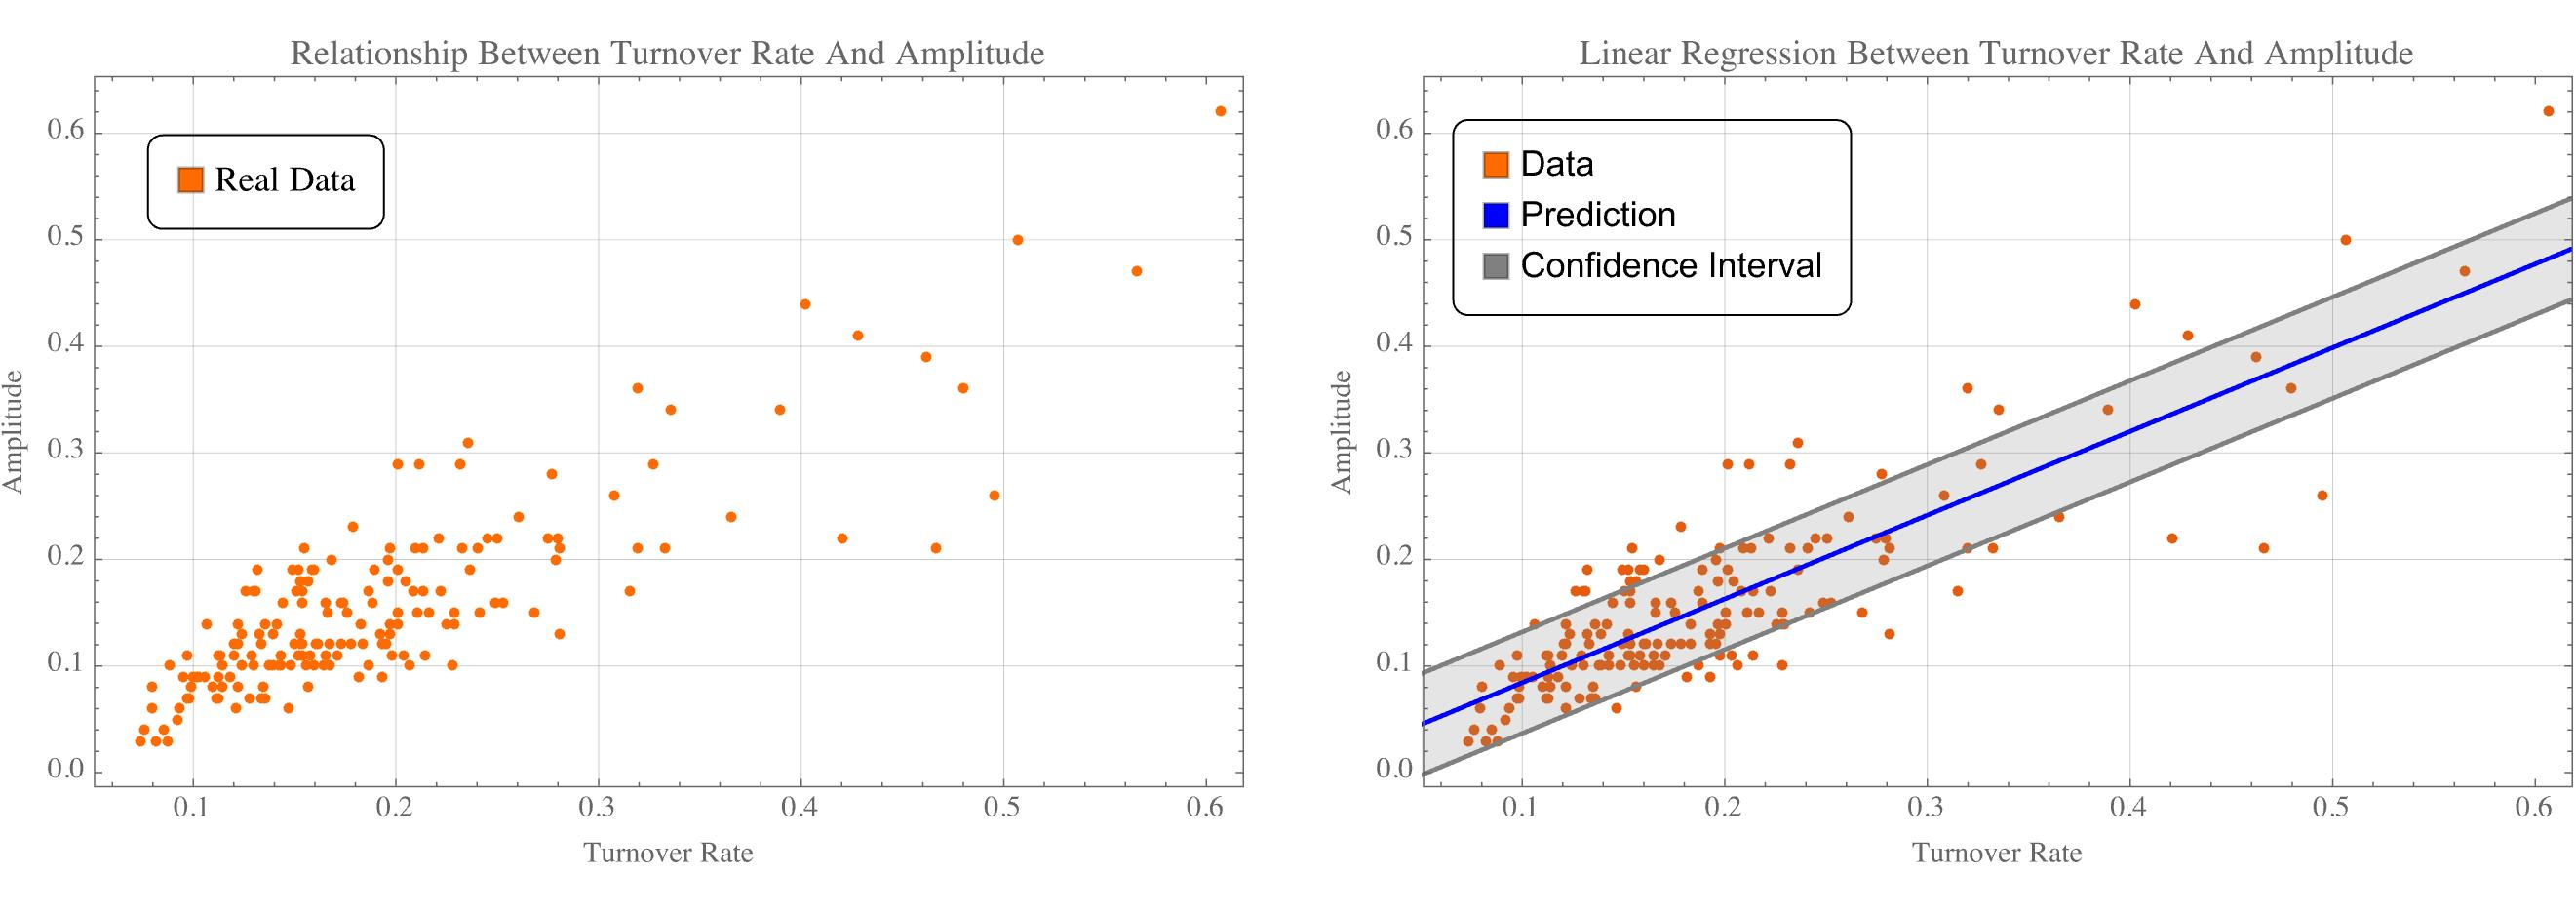
\includegraphics[width=1\textwidth]{linearregression.jpeg}
    \caption{\kaishu 换手率-价格振幅的线性回归}
    \label{fig:turnamp}
\end{figure}

价格振幅与换手率之间的关系大致为
\[
    \text{Amplitude} = 0.00483134 + 0.790811* \text{TurnoverRate}
\]
线性相关系数 $R^2 = 0.894767$ ,拟合良好。这也暗示了换手率对价格波动的影响较为直接,我们希望通过换手率来预测股价的变动,进而通过一定的交易策略实现增值。

\subsection{换手率-时间的自回归模型}

假设换手率与时间的关系为自回归过程,分别取 $k = 3,k = 5,k = 7$ 构造多元线性回归模型,结果如图 \ref*{fig:inone} (c)、(d)所示。可以看到自回归模型的涨跌趋势与真实数据基本一致,符合较好。

从图中可以看出,三组自回归模型的预测峰值大多是超前的,并且预测值在多数情况下低于真实值。这可能是因为我们自回归模型中假设噪声 $\epsilon$ 为白噪声,即服从 $\langle \epsilon(t)\epsilon(t')\rangle  = \lambda \delta_{t,t'}$ ,其中 $\lambda $ 为常数。然而金融数据会受到多种多样的影响,如前几日开盘价与收盘价等等,同时许多不可量化的因素也会在其中施加一定的作用,例如政策变化、交易者的心态以及内部交易等,都会让市场产生一些复杂的、匪夷所思的变化。

这样一来,我们最开始的假设“股价在第 $i$ 天内的变化服从漂移为 $\mu_i$  和方差 $\sigma_i$  一定的维纳过程”就有些许不合理之处。为了减少这一问题造成的麻烦,我们可以使用更高级的金融分析工具,比如伊藤过程或者莱维飞行来近似这种非理性因素所造成的对高斯正态假设的偏离。

不过,我们总是可以通过经验对模型做一些调整,例如给预测结果乘上一定的倍数,并作用一定量的水平位移,使得预测结果与真实数据更为接近。





\begin{figure}[ht]
    \centering
    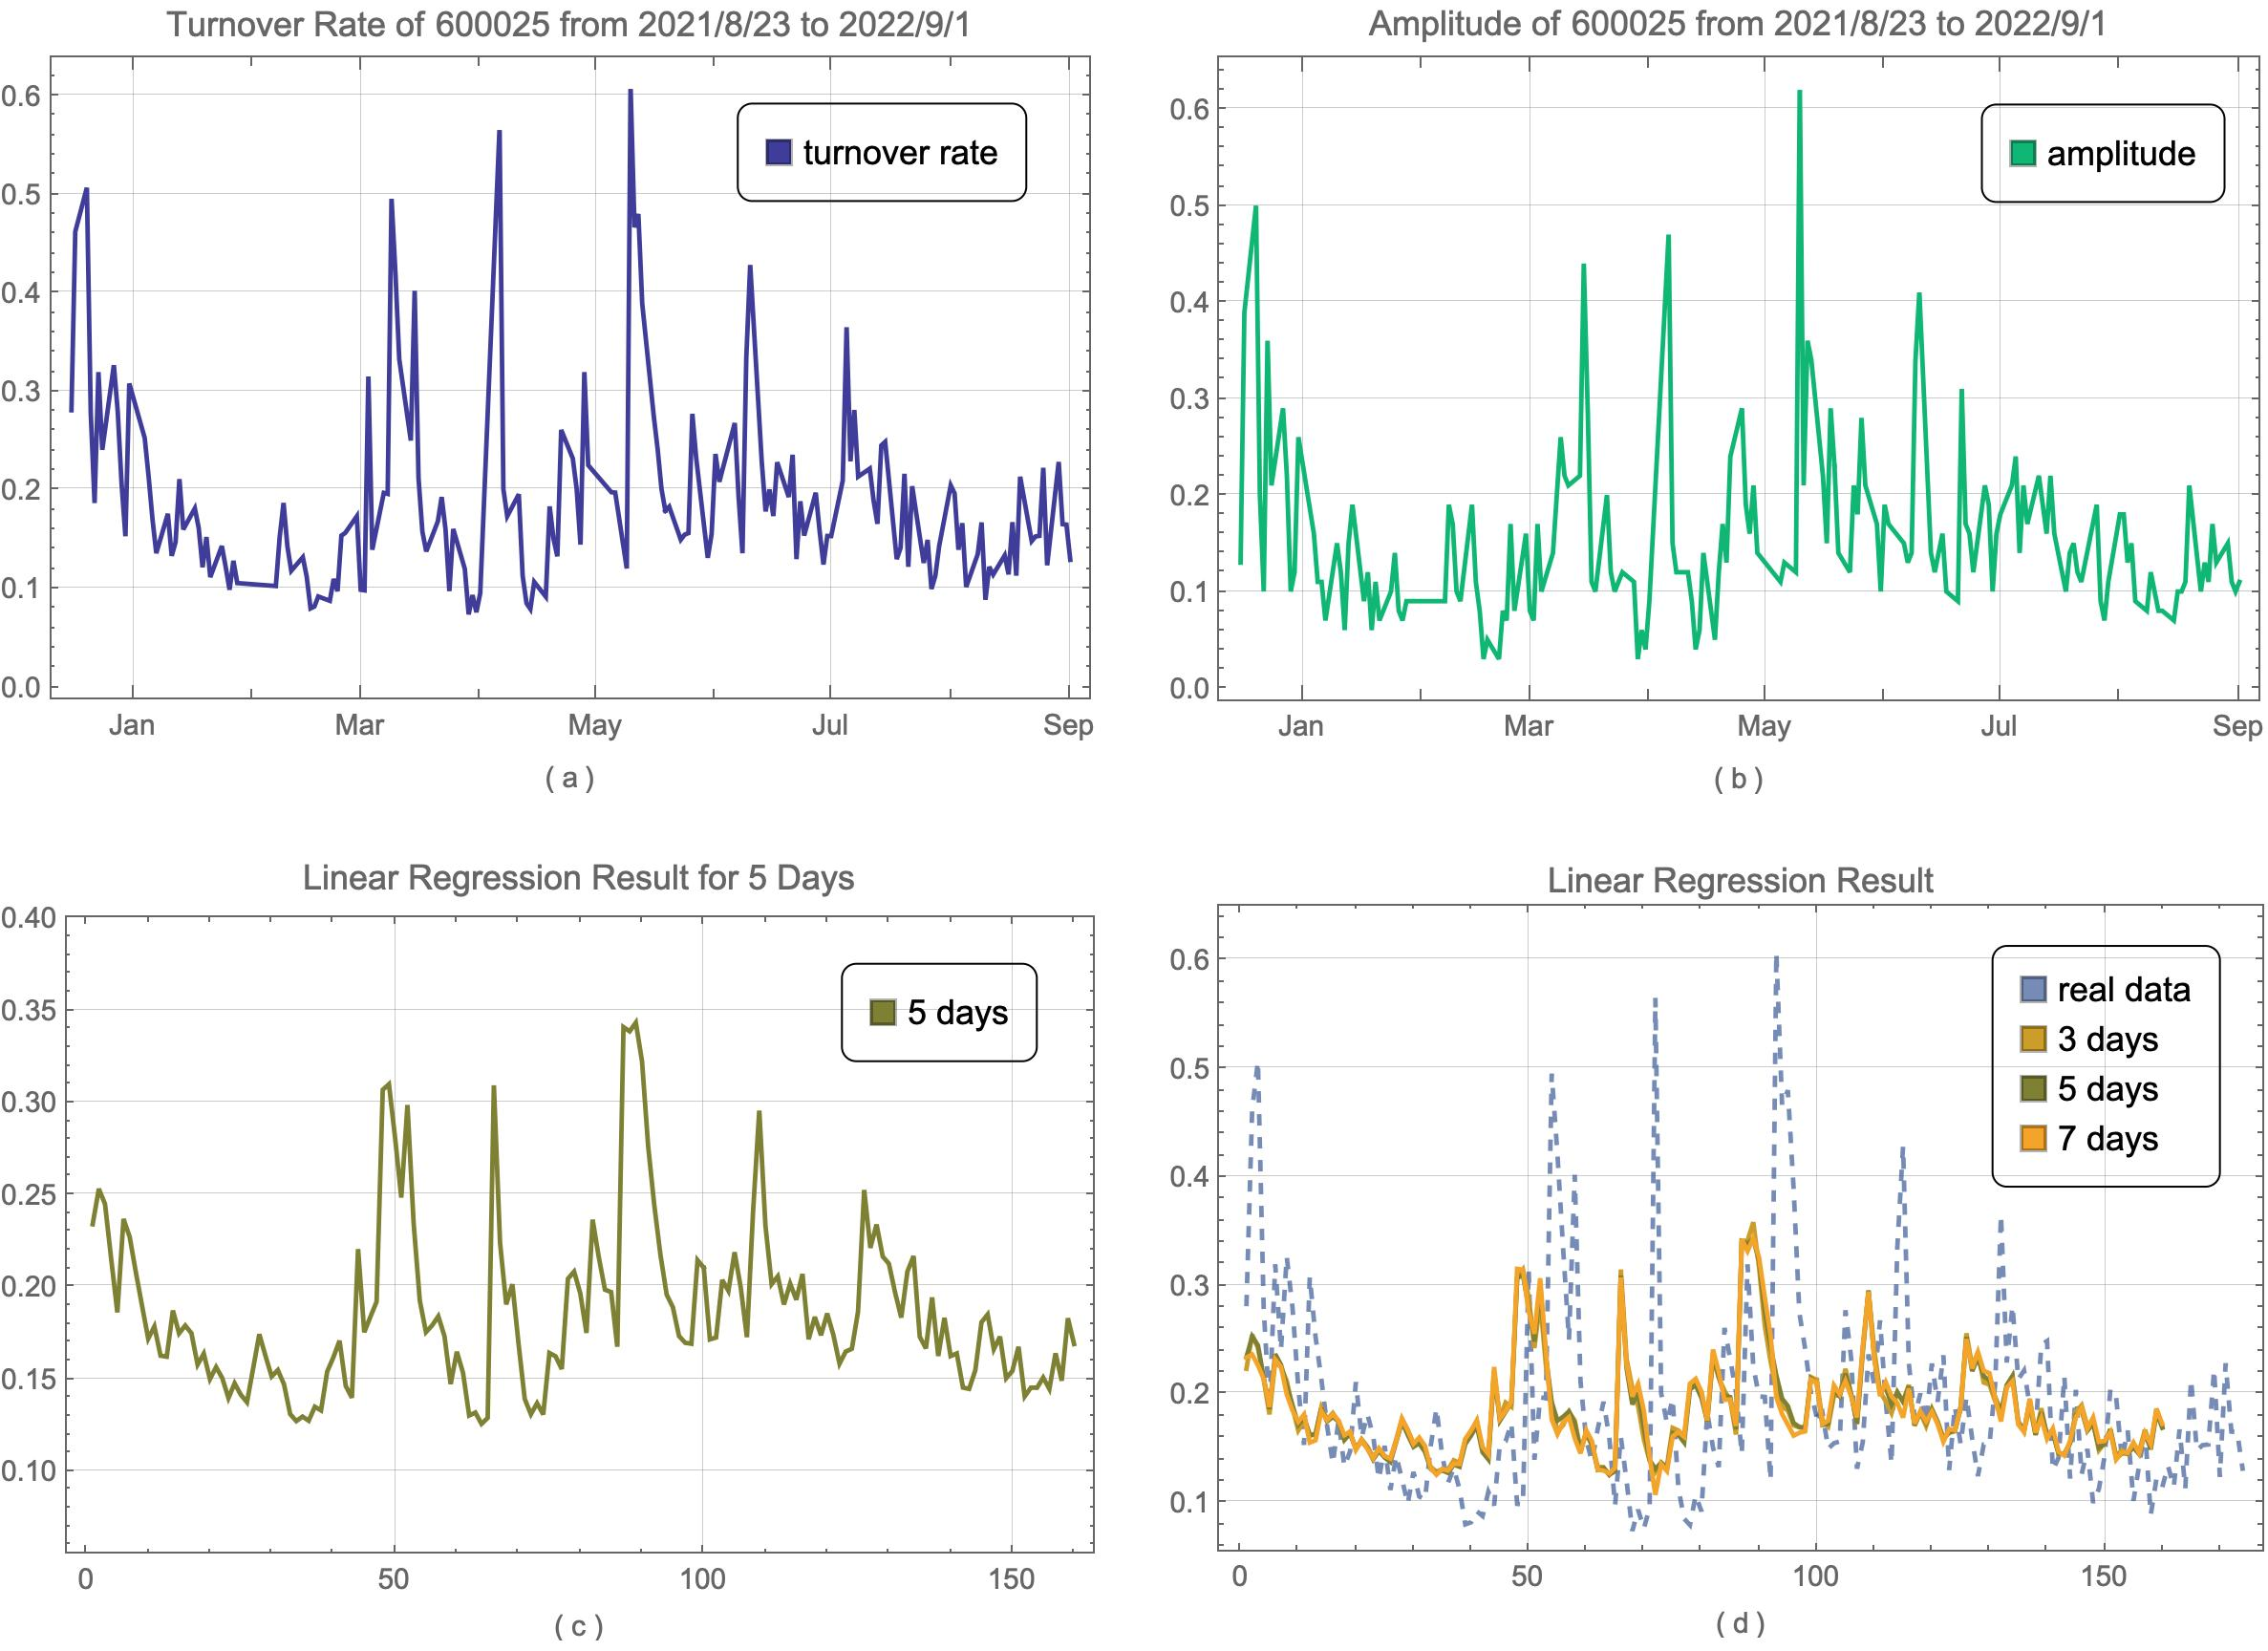
\includegraphics[width=1\textwidth]{inone.jpeg}
    \caption{\kaishu (a):600025 在2021年8月23日与2022年9月1日之间的换手率数据\;(b):600025 在2021年8月23日与2022年9月1日之间的价格振幅数据\;(c):五阶自回归模型的预测结果\;(d):三阶、五阶与七阶自回归模型结果与真实数据对比}
    \label{fig:inone}
\end{figure}

\pagebreak

\subsection{蒙特卡洛法优化自回归参数}

基于对换手率的自回归预测,我们制定了一定的交易策略以期从股市中获利。经过一定的数字实验,选择四阶自回归模型

\[
    x_{n+4} = a_1x_{n-1} + a_2x_{n-2} + a_3x_{n-3} + a_4x_{n-4} + \epsilon
\]
编写交易策略的 C 语言程序,并使用 WSTP 接口与 Mathematica 建立连接,使得 C 语言程序在 Mathematica 中可以作为函数调用,其在 Mathematica 中的名称为 Algorithm3[],参见随文附件。

将生成的随机参数导入交易策略函数并输入历史数据,可以得到这些参数组合对应的收益情况。按照收益从高到低的顺序,我们将参数分为“good”($15\%$)、 “medium”($15\% \backsim 40\%$) 以及 “bad”($40\% \backsim 100\%$),利用 Mathematica 自带的 Classify[] 函数,我们可以使用机器学习方法对这些数据进行学习,并得到对应的模型,使得它能够判断一个新的参数组合的表现情况,结果如图 \ref*{fig:learningresult} 所示。

\begin{figure}[ht]
    \centering
    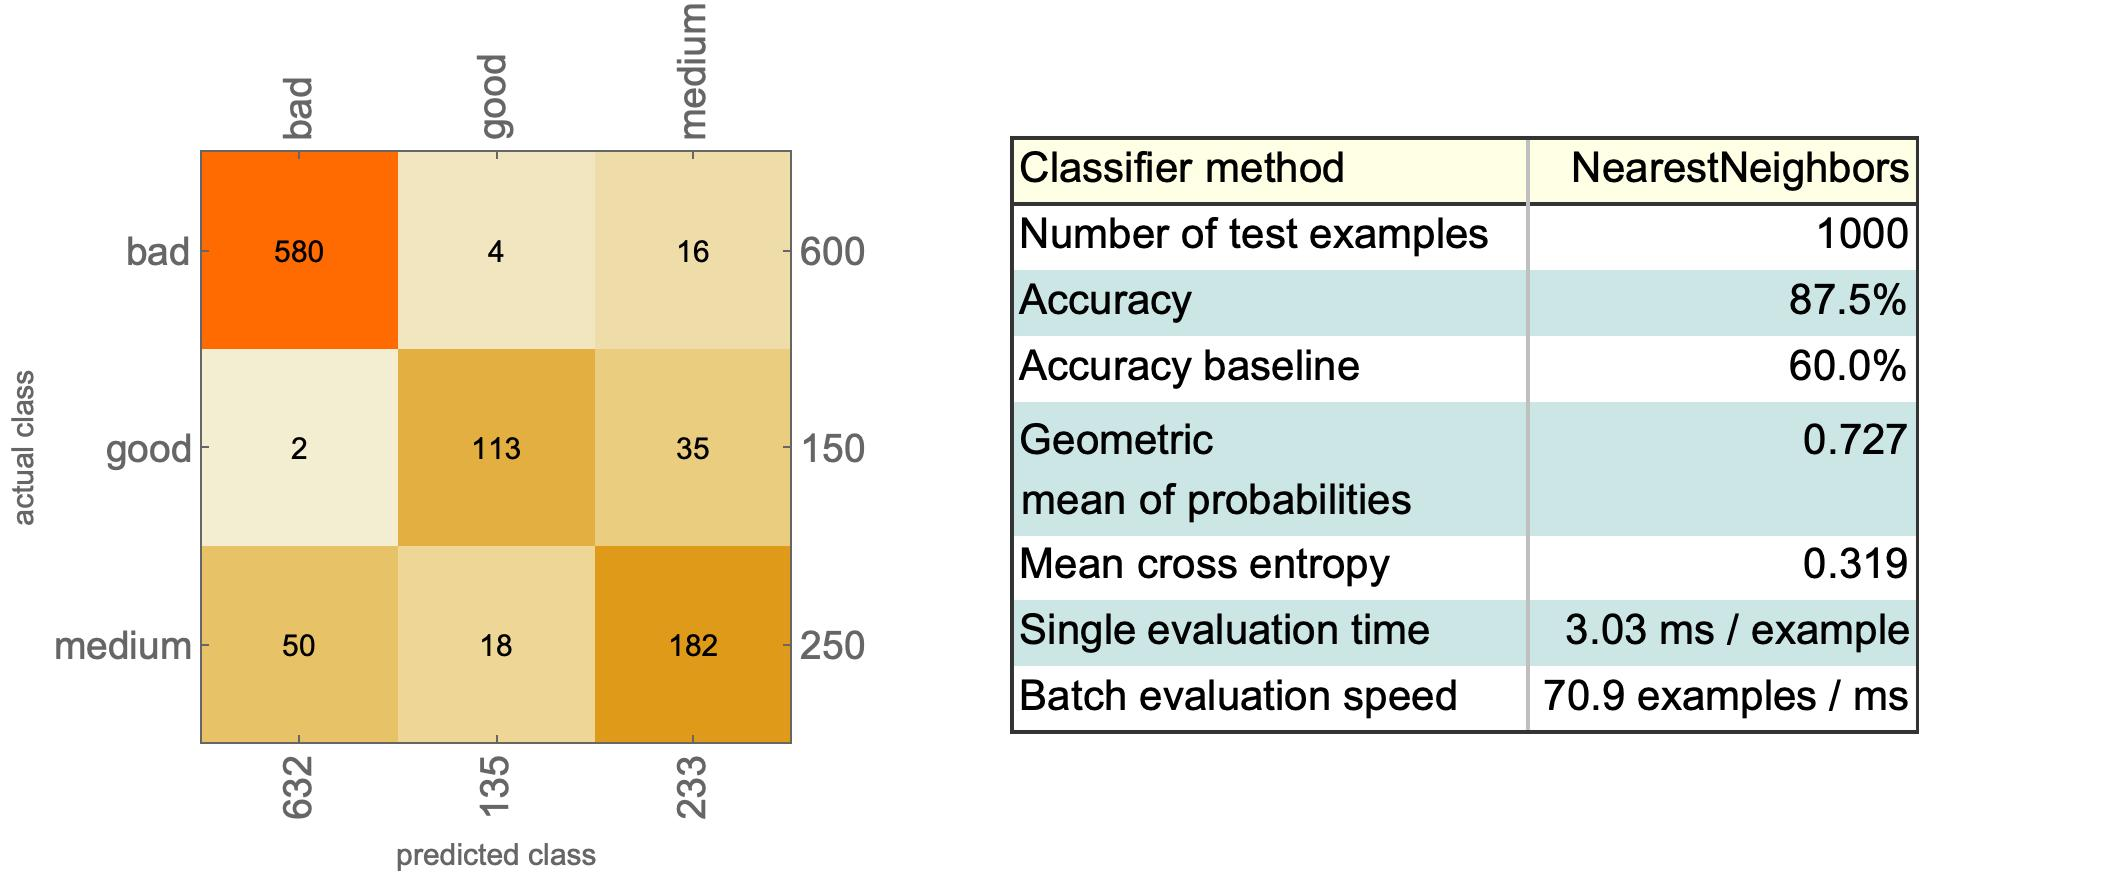
\includegraphics[width=1\textwidth]{learningresult.jpeg}
    \caption{\kaishu 混淆矩阵与模型主要度量}
    \label{fig:learningresult}
\end{figure}

Mathematica 的计算结果表明,使用 NearestNeighbours 的学习算法表现最佳,这也符合我们的预期:参数空间是连续变化的,距离较近的参数点,它们的表现应当接近。

我们的分类对于 bad 类型的参数的准确度高达 $91.7\%$ ,说明这些参数有更多的相似性,可以被很好的分类。但对于 medium 以及 good 型的参数,分类准确度分别为 $83.7\%$ 与 $78.1\%$ ,比较模糊。这也反映了金融系统的复杂性,使得我们无法准确地得到最赚钱的那个方法。

以2022年1月1日至2022年11月10日的数据构建模型,本算法给出的最佳自回归参数为
\[
    a_1=0.512242,\;a_2=0.31025, \;a_3=0.08961 ,\;a_4=0.0878976
\]
这些参数的值每一天都在不断变化,但大体趋势是服从 $a_1>a_2>a_3>a_4$ 。这也表明前几日的情况对今日数据的影响随时间间隔的增加而逐渐减弱。


截止到2022年11月14日,我们已经使用此模型计算得到的参数配比创收了 132.4 元人民币。


\section{总结与展望}

本文利用 Mathematica 完善的金融数据库以及优良的机器学习算法,通过引入简单的时间序列假设,研究了股票换手率与当日振幅的线性关系,并验证了自回归模型在换手率预测中的有效性。在此基础上,我们使用蒙特卡洛方法对一个基于自回归模型交易策略进行了自回归参数的调整与优化。

我们发现,一支股票的当日振幅与当日换手率有明显的线性关系,这应归结于换手率的升高使得时间序列的标准差变大,从而增加了一维维纳过程的方均位移。

然而,自回归模型应用于换手率的预测时的效果欠佳,并且增加参加线性回归的前序天数无助于提高预测准确度,这可能是因为我们的假设本身较为保守,在换手率的突变的位置就会失真。

最后,利用蒙特卡洛方法,我们对一个基于自回归模型的交易策略的经验参数进行了调整与优化,使得将该策略应用于去年至今的历史数据时的收益率稳定在 22\% 左右,相比手动调整的方法效率有所提升。

未来我们将应用更专业的 Fama-French 资本资产定价模型,将市场风险、市值风险和账面市值比风险作为因子来预测上市公司股票收益变化。进而从股市中获得更高的超额收益。此外,本文一些结果还表明,维纳过程由于它过于理想的假设,在模拟金融数据上并不优良。对此应当考虑用莱维飞行或者伊藤过程进行替代。

\section{声明}

本文使用的Mathematica 源程序、C语言源程序以及 WSTP 端口代码参见随文附件。

机器学习模型已上传至 Wolfram Cloud ,公开链接为 \href{https://www.wolframcloud.com/obj/617a368e-36b5-4bb7-b4dc-ea6a933ed0f6}{\kaishu 自回归参数分类模型},相应 api 以及 C 语言嵌入代码见附录。


\section{致谢}

本文使用的 C 语言源程序由中国科学技术大学化学物理系周雨函同学编写,他在分析投资时展现的非凡洞察力以及敢于冒险的勇气都给我们极大的鼓励。

\pagebreak
\bibliographystyle{plain}
\bibliography{ref}

\pagebreak

\kaishu

\section*{\kaishu\LARGE\bfseries{附录I~~~证明方均位移的期望与标准差成正比}}

    对于标准布朗运动 $B(t)$,$\mu = 0,\sigma^2 = 1$。记$B(t_k)-B(t_{k-1}) = \Delta B(k),\;(k=1,2,\dots,n)$,则$\Delta B(k)\thicksim N(0,\Delta t_k)$,且$E\left[\Delta B(k)^2\right] = \Delta t_k,\;\;E\left[\Delta B(k)^4\right] = 3 (\Delta t_k)^2,\;\;(k=1,2,\dots,n)$,对差的平方求期望,根据增量的独立性:
    \begin{align*}
        E\left[B(t)^2 - t\right]^2 &= E\left[\sum_{k=1}^n (\Delta B(k)^2 -\Delta t_k) \right]^2  \\
        &= \sum_{k=1}^n E\left[\Delta B(k)^2 -\Delta t_k \right]^2     \\
        &= \sum_{k=1}^n \left[E\Delta B(k)^4 -2\Delta t_k * E\Delta B(k)^2 + (\Delta t_k)^2 \right] \\
        &= \sum_{k=1}^n \left[3 (\Delta t_k)^2 -2(\Delta t_k)^2 + (\Delta t_k)^2 \right]\\
        &= 2\sum_{k=1}^n (\Delta t_k)^2
    \end{align*}
    设 $\lambda = \text{max}\;\Delta t_k \rightarrow 0$ ,则有
    \begin{align*}
        2\sum_{k=1}^n (\Delta t_k)^2 &\leq 2 \lambda \sum_{k=1}^n \Delta t_k \\
        &= 2 \lambda t \rightarrow 0
    \end{align*}  

    \pagebreak

    \section*{\kaishu\LARGE\bfseries{附录II~~~C语言嵌入程序}}
    \lstset{
        breaklines,                                 % 自动将长的代码行换行排版
        extendedchars=false,                        % 解决代码跨页时,章节标题,页眉等汉字不显示的问题
        backgroundcolor=\color[rgb]{0.96,0.96,0.96},% 背景颜色
        keywordstyle=\color{blue}\bfseries,         % 关键字颜色
        identifierstyle=\color{black},              % 普通标识符颜色
        commentstyle=\color[rgb]{0,0.6,0},          % 注释颜色
        stringstyle=\color[rgb]{0.58,0,0.82},       % 字符串颜色
        showstringspaces=false,                     % 不显示字符串内的空格
        numbers=left,                               % 显示行号
        numberstyle=\tiny,                    % 设置数字字体
        basicstyle=\small,                    % 设置基本字体
        captionpos=t,                               % title在上方(在bottom即为b)
        frame=single,                               % 设置代码框形式
        rulecolor=\color[rgb]{0.8,0.8,0.8},         % 设置代码框颜色
    }
\begin{lstlisting}[language=C]
using System;
using System.Net;
using System.Text;
using System.IO;
using System.Collections.Specialized;

namespace RequestTest
{
	class MainClass
	{

		public static String call(double ratio1, double ratio2, double ratio3, double ratio4)
		{
			using (var client = new WebClient())
			{
    			client.Headers.Add("Content-Type","application/x-www-form-urlencoded");
				client.Headers.Add("User-Agent","EmbedCode-CSharp/1.0");
				
				string postData="";	
				postData +=  "ratio1" + "=" + ratio1 + "&";postData +=  "ratio2" + "=" + 
                ratio2 + "&";postData +=  "ratio3" + "=" + ratio3 + "&";postData +=  
                "ratio4" + "=" + ratio4 + "&";
				
				byte[] byteArray = Encoding.ASCII.GetBytes(postData);
				string url = "http://www.wolframcloud.com/obj/ustcxkc/GoodBadPredictor";
				var response = client.UploadData(url, byteArray);

   				var responseString = Encoding.Default.GetString(response);
				client.Dispose();
				
        		return responseString;

			}
		}
	}
}
\end{lstlisting}


\section*{\kaishu\LARGE\bfseries{附录III~~~其他附图}}

\begin{figure}[ht]
    \centering
    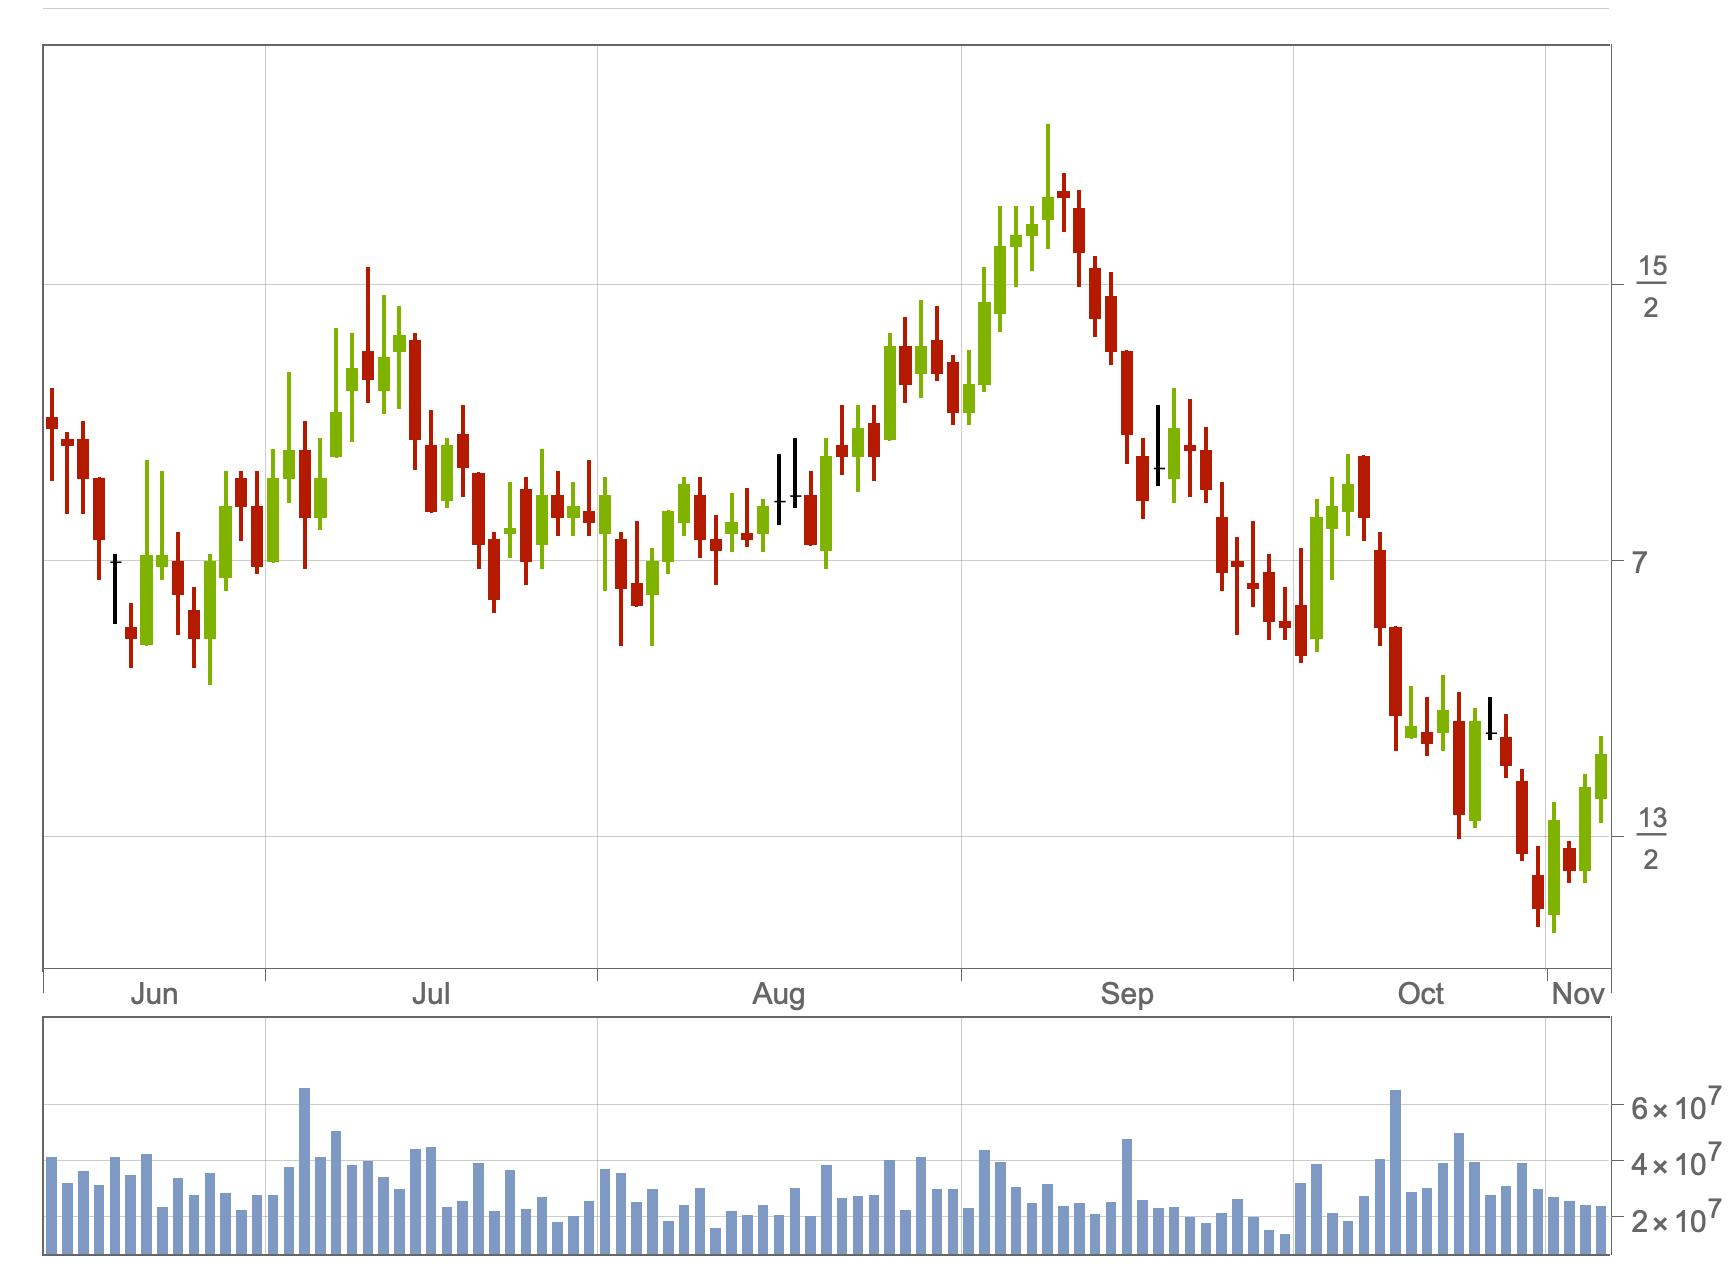
\includegraphics[width=1\textwidth]{stoke.jpeg}
    \caption{\kaishu600025最近250日的股价数据}
    \label{fig:stokes}
\end{figure}

\begin{figure}[ht]
    \centering
    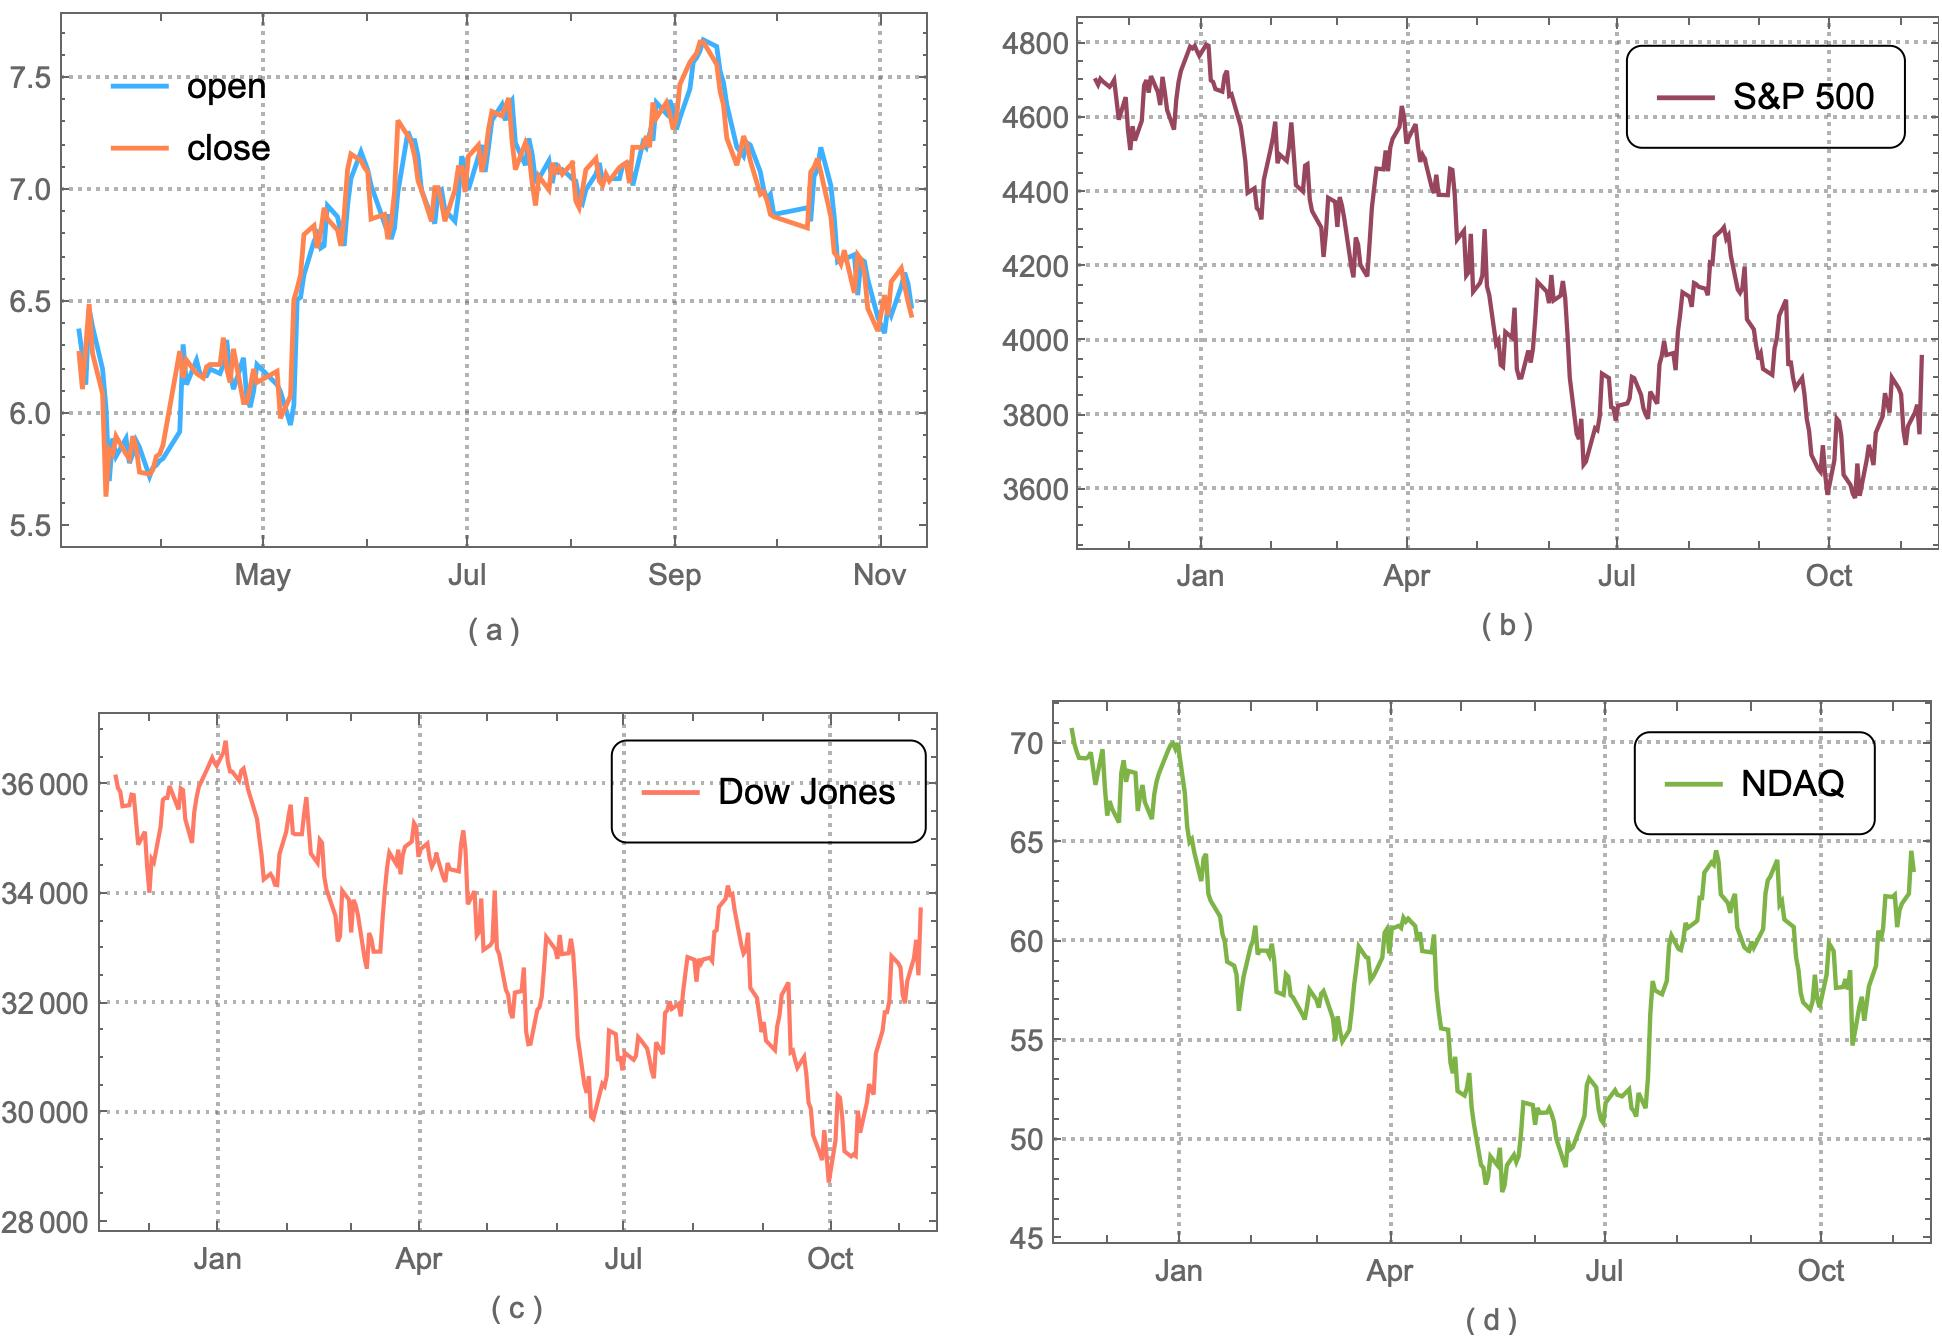
\includegraphics[width=1\textwidth]{sanda.jpeg}
    \caption{\kaishu (a):600025 在2021年8月23日与2022年9月1日之间的开盘价与收盘价数据\;(b):标准普尔 500 最近250日的数据\;(c):道琼斯工业指数最近250日数据\;(d):纳斯达克指数最近250日数据}
    \label{fig:引用标签}
\end{figure}

\begin{figure}[ht]
    \centering
    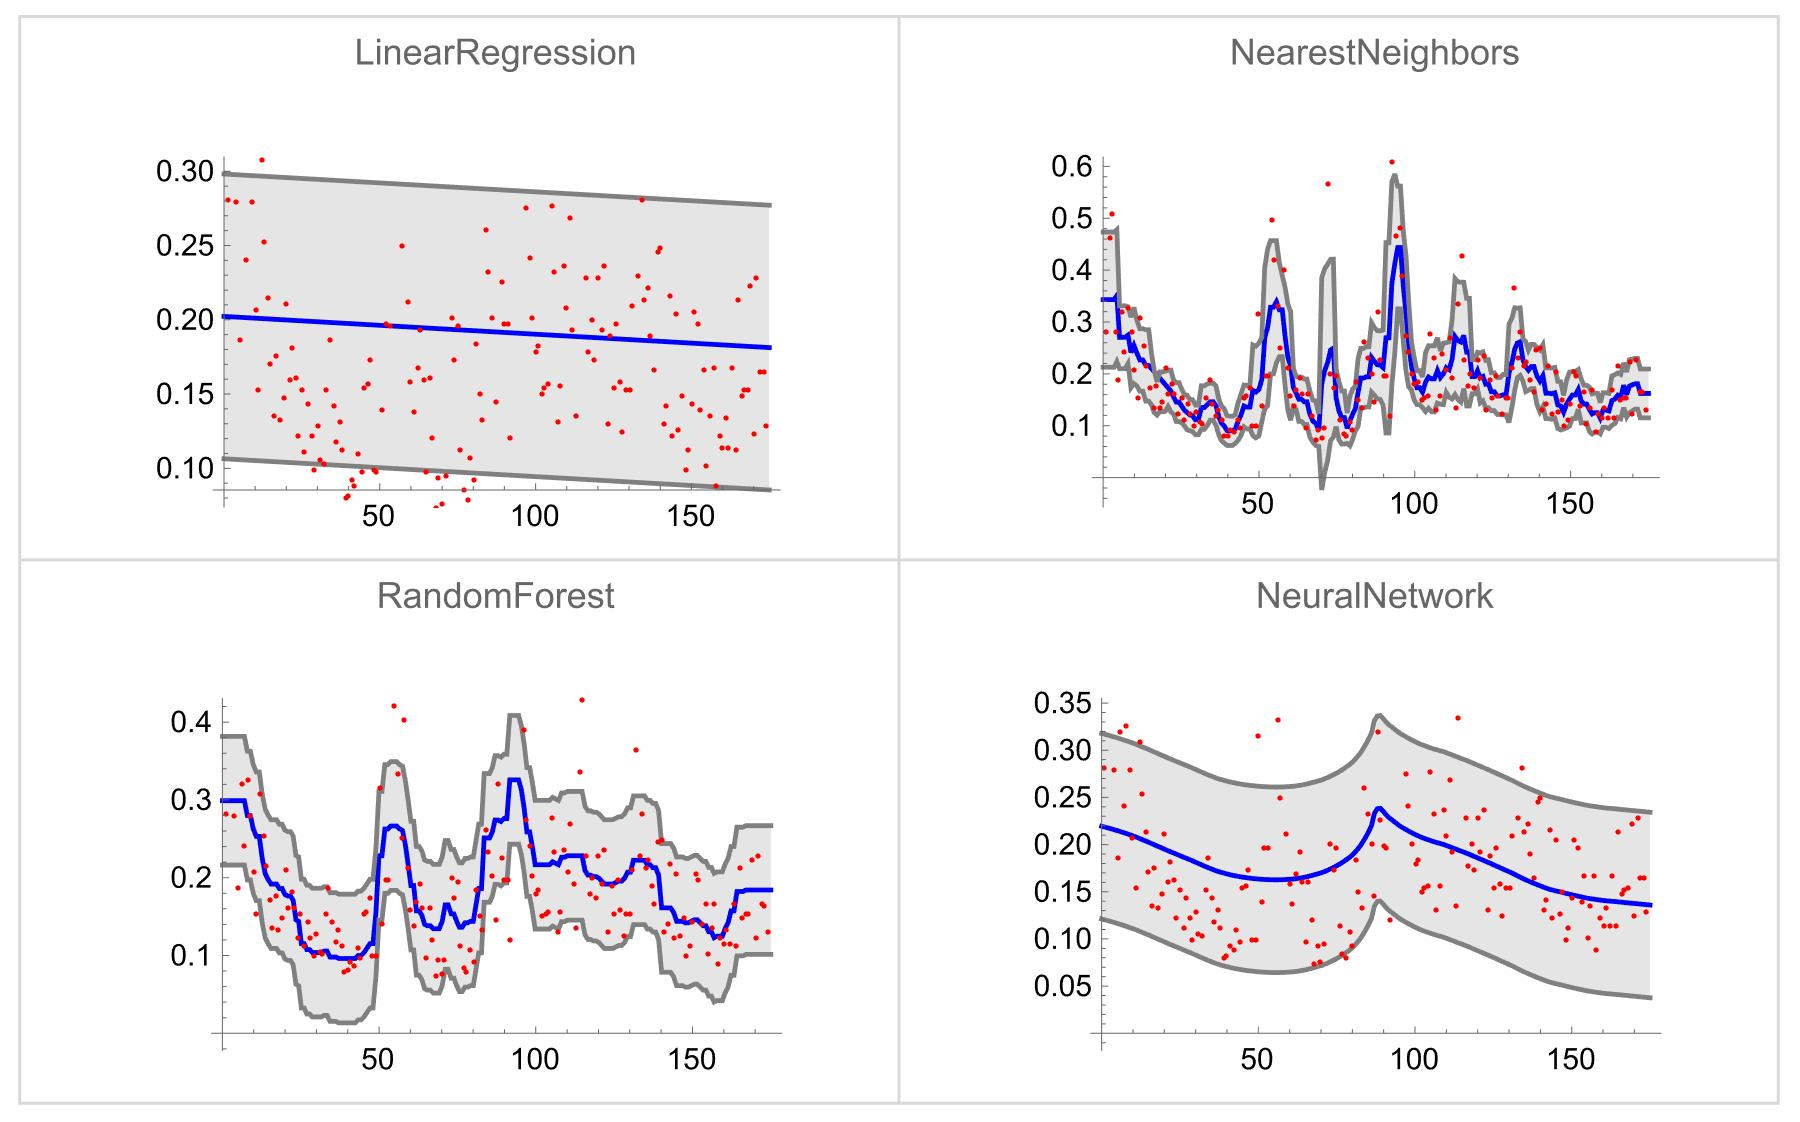
\includegraphics[width=1\textwidth]{learn.jpeg}
    \caption{\kaishu 直接将每日换手率数据输入 Predict[] 的学习结果}
    \label{fig:learnfail}
\end{figure}


\end{document}


